%%%%%%%%%%%%%%%%%%%%%%%%%%%%%%%%%%%%%%%%%%%%%%%%%%%%%%%%%%%%%%%%%%%%%%%%%%%%%%%%
%2345678901234567890123456789012345678901234567890123456789012345678901234567890
%        1         2         3         4         5         6         7         8

\documentclass[letterpaper, 10 pt, conference]{ieeeconf}  % Comment this line out if you need a4paper

%\documentclass[a4paper, 10pt, conference]{ieeeconf}      % Use this line for a4 paper

\IEEEoverridecommandlockouts                              % This command is only needed if
                                                          % you want to use the \thanks command

\overrideIEEEmargins                                      % Needed to meet printer requirements.

%In case you encounter the following error:
%Error 1010 The PDF file may be corrupt (unable to open PDF file) OR
%Error 1000 An error occurred while parsing a contents stream. Unable to analyze the PDF file.
%This is a known problem with pdfLaTeX conversion filter. The file cannot be opened with acrobat reader
%Please use one of the alternatives below to circumvent this error by uncommenting one or the other
%\pdfobjcompresslevel=0
%\pdfminorversion=4

% See the \addtolength command later in the file to balance the column lengths
% on the last page of the document

% The following packages can be found on http:\\www.ctan.org
\usepackage{graphicx} % for pdf, bitmapped graphics files
%\usepackage{epsfig} % for postscript graphics files
%\usepackage{mathptmx} % assumes new font selection scheme installed
%\usepackage{times} % assumes new font selection scheme installed
\usepackage{amsmath} % assumes amsmath package installed
\usepackage{amssymb}  % assumes amsmath package installed
%\usepackage{dsfont}
\usepackage{algorithm}
\usepackage{algorithmic}
\usepackage{commath}

\usepackage{xcolor}
\newcommand{\todo}[1]{{\color{blue}[TODO: #1]}}
\newcommand{\response}[1]{{\color{green}[RESPONSE: #1]}}

\DeclareMathOperator*{\argmax}{arg\,max}
\DeclareMathOperator*{\argmin}{arg\,min}

\title{\LARGE \bf
Optimal Coverage with Genetic Path Planning
}


\author{Jacob M. Olson, Craig C. Bidstrup$^{1}$, Brady K Anderson,Which Professors?$^{2}$% <-this % stops a space
\thanks{This research was supported through the Center for Unmanned Aircraft Systems (C-UAS), a National Science Foundation-sponsored industry/university
cooperative research center (I/UCRC) under NSF Award No. IIP-1650547
along with significant contributions from C-UAS industry members.}% <-this % stops a space
\thanks{$^{1}$The corresponding author can be contacted at
        {\tt\small craig.bidstrup at byu.edu}.}%
\thanks{$^{2}$All authors are with the Department of Mechanical Engineering or Electrical and Computer Engineering,
        Brigham Young University, Provo, UT, 84602, USA.}%
%\thanks{$^{3}$C. Peterson is with the Faculty of Electrical and Computer Engineering,
%		Brigham Young University, Provo, UT, 84602, USA.
%        {\tt\small cammy.peterson at byu.edu}}%
%\thanks{$^{4}$R. W. Beard is with the Faculty of Electrical and Computer Engineering,
%		Brigham Young University, Provo, UT, 84602, USA.
%        {\tt\small beard at byu.edu}}%
}



\begin{document}



\maketitle
\thispagestyle{empty}
\pagestyle{empty}


%%%%%%%%%%%%%%%%%%%%%%%%%%%%%%%%%%%%%%%%%%%%%%%%%%%%%%%%%%%%%%%%%%%%%%%%%%%%%%%%
\begin{abstract}

When generating 3D maps with unmanned arial vehicles (UAVs), it is important to the mapping algorithms to have good coverage of the environment and have multiple loop closures throghout the flight path. Because multirotor UAVs are limited in flight time, the flight paths must not be too long. Coming up with a good flight path of a new environment to be mapped can be difficult to do well and becasue of how free-form a flight path can be, it is also tricky to generate optimal paths to get good coverage with minimal flight time.
to solve this problem, we propose using a genetic algorithm designed to maximize total area coverage while minimizing flight time. Because of the more randomized searching that genetic algorithms have, it is more capable of solving complex free-form problems like path planning.

\end{abstract}


%%%%%%%%%%%%%%%%%%%%%%%%%%%%%%%%%%%%%%%%%%%%%%%%%%%%%%%%%%%%%%%%%%%%%%%%%%%%%%%%
\section{INTRODUCTION}

Talk about lit review and what we will be contibuting to the space

The remainder of the paper is organized as follows: Section \ref{setup} describes the method for simplifying the design space to create a reasonable problem for the genetic algorithm to solve. Section \ref{approach} describes the approach and architecture used to generate optimimal paths for first, a single UAV, then the method is extended to multi-agent path planning. Results showing and evaluating the generated paths are presented in Section \ref{results}. Finally, conclusions are presented in Section \ref{conclusions}.

%%%%%%%%%%%%%%%%%%%%%%%%%%%%%%%%%%%%%%%%%%%%%%%%%%%%%%%%%%%%%%%%%%%%%%%%%%%%%%%%
\section{OPTIMIZATION SETUP}\label{setup}

With optimization, especially genetic algorithms, it is important to have a problem that is high enough fidelity to model a problem close enough to the real world that it is useful, but simplified enough that it is able to make progress and learn between generation so that it is able to run.

\subsection{Problem Statement}

The problem being solved by this genetic algorithm is generating paths through a simple floor plan to be able to generate a 3D map with a UAV when the planned flight paths are flown. To do this, we start with a simple floor plan of the area that we want to map and a known scale of the map, then with as little required human interaction as possible, the goal is to generate a flight paths for the desired ammount of agents to map the building as well as possible with short enough flight times that it will be feasible with real hardware.

\subsection{Discretization}

The first step of setting up the optimization is making sure that the problem can be solved. because of the very open-ended nature of path planning, we needed to find a way to discretize and simplify the space to make this a solvable problem.

\subsubsection{Map Generation}

To do this, we started with the simple 2D floor map that we are starting with. 2D floor maps are very accessible for most buildings, so it is a reasonable place to start. the only part of the genetic algorithm that must be manually done by a human before starting the optimization is finding a floor map and masking it with areas that you want to map and areas that you do not want to map. Fig. \ref{fig:map_gen} illustrates what this mask would look like. The white space is flyable area, and the black space is unflyable space such as walls or inaccessible rooms.

\begin{figure}
\centering
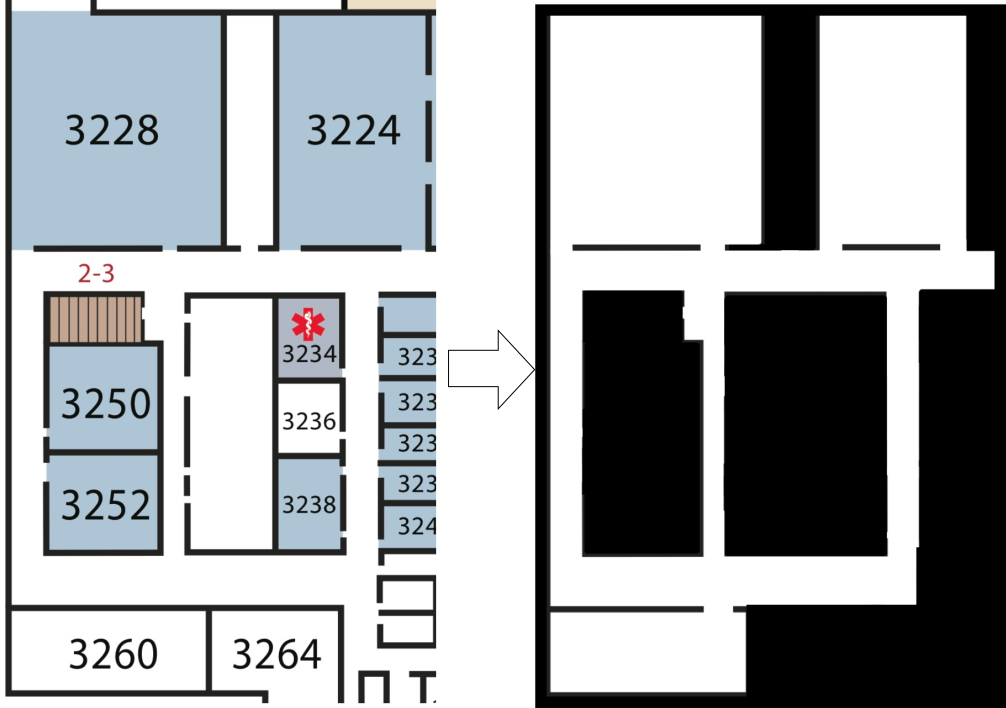
\includegraphics[width=0.8\linewidth]{figures/map_bw.png}
\caption{The initial two dimensional floor map of the area to be mapped and the altered floor map reflecting areas that are to be mapped and areas that can be ignored}
\label{fig:map_gen}
\end{figure}

Once this map is generated, it is used to begin the algorithm along with the scale from pixels to meters and the width of the narrowest hallway (in meters).

The map generator then takes the masked map and scales it down so that each pixel represents the minimum resolution desired in the optimization. In our case, we scaled it to $0.15 m^{2}$ per pixel. This value could be adjusted to either increase the fidelity of the planner, or decrease it to make the optimization run faster.

\subsubsection{Waypoints}

Once the map is scaled to the desired size, to further discretize and simplify the design space of the optimization, We placed waypoints on the map and contrained the flight path to only fly through these waypoints. the first step of generating the waypoint is to lay down a grid of waypoints spaced apart by one half the width of the narrowest flyable hallway on the map to ensure that there are waypoints in every hallway and in every room so that the UAV can get everywhere it needs to to map the environment. After placing the grid of waypoints, all waypoints in unflyable space are removed.

After removing waypoints that were in unflyable space, the waypoints are further pruned and adjusted to better represent the flyable space, the first step is to calculate a safety buffer around all unflyable space where the UAV will be able to fly without colliding with walls. Any waypoint that falls in this safety buffer is nudged out of it. Then waypoints are pruned one last time to remove redundant waypoints. This is done by checking the distance between waypoints. Any waypoints that are closer to eachother than the initial grid separation (one half the width of the narrowest hallway) are adjusted and pruned. If a waypoint is too close to only one other waypoint it is moved, half the distance to the other waypoint and then the other one is removed. An example of this is point A in Fig. \ref{fig:waypoints}. If a waypoint is too close to multiple other waypoints, it stays where it is and the other waypoints are removed. An example of this is point B in Fig. \ref{fig:waypoints}. This prevents over crowding of waypoints in halways and corners to make it simpler to generate flight paths through narrow hallways and near walls in rooms. Fig. \ref{fig:waypoints} shows how this step would work.

\begin{figure}
\centering
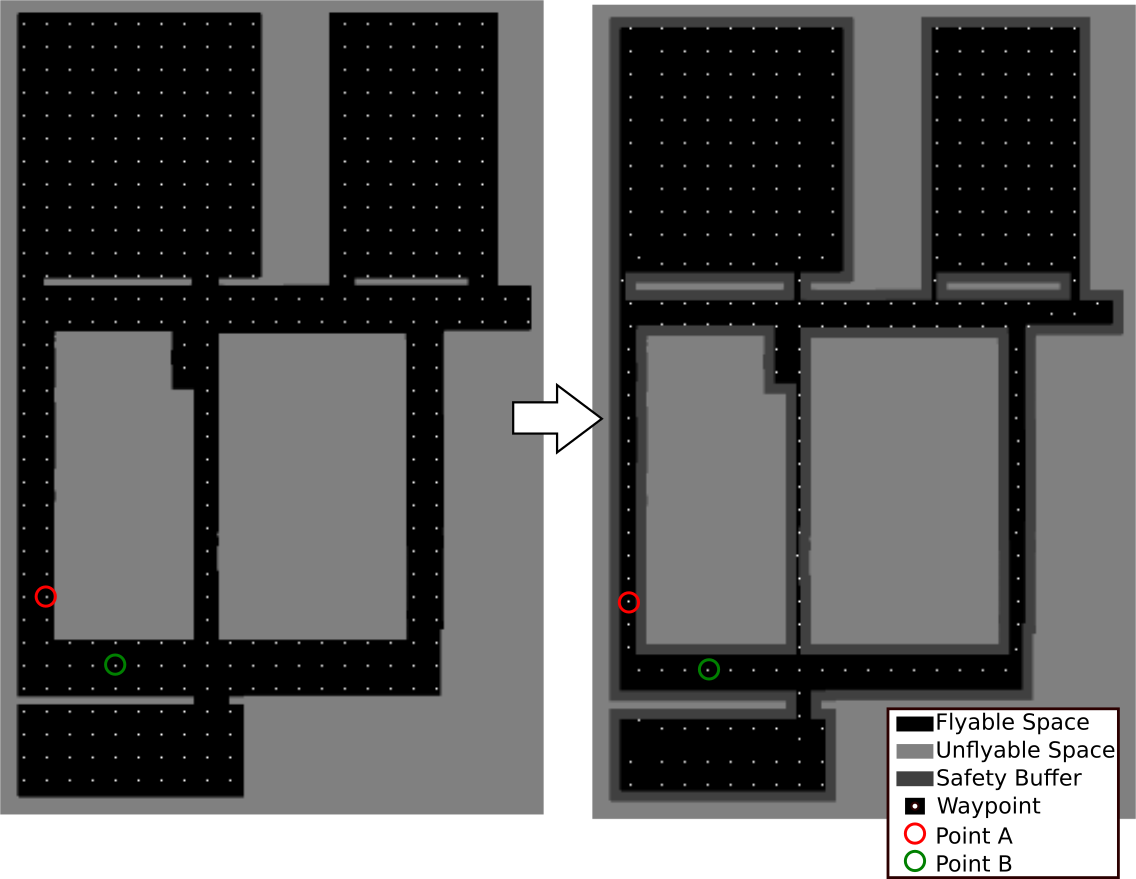
\includegraphics[width=0.8\linewidth]{figures/waypoint2.png}
\caption{The initial waypoint grid with only waypoints on unflyable space removed on the left, The modified waypoint grid with safety buffer and anti-crowding on the right.}
\label{fig:waypoints}
\end{figure}

\subsection{Objective Functions}

The goal of this optimization is to generate paths that get good coverage of the environment so that the UAVs can generate good 3D maps. Since this problem is constrained to flight paths of UAVs it is also important to not generate paths that are too long, which would not be possible to fly in a single flight with a UAV. To compensate for this, we decided to create a genetic algorithm with two competing objectives.

\subsubsection{Maximize Coverage}

The first objective is to maximize coverage of the environment. To compute the coverage we used the parameters for the RGB-D camera that we will use when mapping the environment. We used the parmaeters minimum depth, maximum depth, and horizontal field of view to create a field of view frustum. To simplify the problem, we assumed that the UAV would only fly forward. We then used the frustum at each waypoint on the path and set the pixels inside the frustum to "viewed." After doing that for every waypoint, we divided the total number of viewed pixels by the total number of pixels in flyable space. The value of the coverage was used (percent seen) as the first objective function.

\subsubsection{Minimize Flight Time}

The second objective function was to minimize flight time. To acheive this, we assumed constant velocity and computed the total distance flown in each path. we also modified this to penalize turning by adding a cost proportional to the amount the uav turns between each waypoint. This way, paths with less waypoints and less turns are considered more fit according to the objective function.

\subsection{Traversable Graph}

To save computation when generating new paths or modifying paths, we precomputed the reachable waypoints from each waypoint. For any given waypoint we wanted to constrain movement only to adjacent waypoints that were not obscured by obstacles. To do this, we created a traversablity graph which was matrix with each row representing a waypoint and each column representing every other waypoint, we populated the matrix with ones where the other waypoint is traversable from the current waypoint and zero where it is not. We split up the space around each waypoint into octants, we then found the nearest waypoint in each octant and populated the graph with those possibilities. To prevent flying into obstacles, we pruned the graph to remove any traversing that is obscured by obstacles with a simple line intersection algorithm.

We used this traversablity graph to generate paths for the agents. we passed in the desired path length and the starting location. Then it randomly choses the next waypoint from the traversabilty graph, the probablility is a normal distribution favoring moving forward to prevent too much meandering. also to prevent backtracking, we also encoded a short term memory of length n into the paths so that unless there is no other available action, it will not return to a waypoint it has been to within the last n timesteps

%%%%%%%%%%%%%%%%%%%%%%%%%%%%%%%%%%%%%%%%%%%%%%%%%%%%%%%%%%%%%%%%%%%%%%%%%%%%%%%%
\section{APPROACH}\label{approach}
\subsection{Single Agent Architecture}
\subsubsection{Low-Variance Sampling}

Low-variance sampling is the mechanism used to sort and sample parents in a way that gives organisms with better designs (determined by a maximin fitness) a higher probability of being selected as a parent.

\subsubsection{Chromosome}

The chromosome defining each member in a generation has a maximum of 250 genes. Each gene represents one waypoint in the traversable graph. The first generation of parents is spawned by generating a random path through the 2d map. The first step to create this first generation is to seed the same initial waypoint to each of the 100 organisms in the generation's population. This models the behavior that no matter what else, the doorway to enter the building is always in the same spot on the local 2D hallway map. Thus, whatever random path may be considered most optimal, it must always start at the entrance. Next, each consecutive waypoint is randomly selected by using the current waypoint as an input to the traversable graph, which produces a random next point from its local neighbors. The first generation all receive a maximum length chromosome of 250 waypoints. This length is allowed to vary in crossover \todo{does this happen in mutation now, as well?}, from the max of 250 waypoints to a minimum of 75 waypoints. Once the chromosome is defined, the coverage and flight time objective values are computed for that organism, or design.

\subsubsection{Crossover}

The first generation is treated slightly different in preparation for crossover. In order to get the first set of children, the fitness value for each parent is computed using a maximin comparison with all other members of the first generation. In contrast, all other generations are

\subsubsection{Mutation}
\subsubsection{Constraints}
\subsubsection{Minimax}
\subsubsection{Elitism}


\subsection{Multi-Agent Architecture}
\subsubsection{Low-Variance Sampling}
\subsubsection{Chromosome}
\subsubsection{Crossover}
\subsubsection{Mutation}
\subsubsection{Constraints}
\subsubsection{Minimax}
\subsubsection{Elitism}
%%%%%%%%%%%%%%%%%%%%%%%%%%%%%%%%%%%%%%%%%%%%%%%%%%%%%%%%%%%%%%%%%%%%%%%%%%%%%%%%
\section{RESULTS}\label{results}
\subsection{Single Agent}
\subsubsection{Pareto Front}
\subsubsection{Paths Generated}
\subsection{Multiple Agents}
\subsubsection{Pareto Front}
\subsubsection{Paths Generated}
%%%%%%%%%%%%%%%%%%%%%%%%%%%%%%%%%%%%%%%%%%%%%%%%%%%%%%%%%%%%%%%%%%%%%%%%%%%%%%%%
\section{CONCLUSIONS}\label{conclusions}

Multiple target tracking has a wide array of applications ranging from air traffic control \cite{Li1993} to following shoppers in a store \cite{Liu2007}. Many approaches exist to track moving objects, vehicles, pedestrians, etc. Algorithms of particular interest include Multiple Hypothesis Tracking (MHT) \cite{Reid1979}, Probability Hypothesis Density (PHD) filters \cite{Clark2007}, Recursive RANSAC (R-RANSAC) \cite{Niedfeldt2014}, and their variants. Most applications of these algorithms constrain the area of interest to the field of view of whatever sensor is employed. Targets that move out of the field of view are usually forgotten and considered a new target when seen again.

Other research, where the area of regard is larger than the field of view of an agent's sensor, sometimes pose the situation as a search problem, as in \cite{Allik2017} and \cite{Wong2005}. It has been shown that incorporating additional information, such as road network information, improves the estimate of target state \cite{Cheng2007}. Another powerful technique, employed by \cite{Allik2017} and \cite{Ahmed2017}, is to incorporate negative information. Traditional localization would only update the target location belief if it were viewed. However, if the target is nowhere to be seen within the agent's field of view, this still gives some information as to where it could be.

As an illustration, consider the case where a target could be in one of two possible locations. Searching one will reveal that the target is indeed there or must be at the other location. This sort of negative information update proves valuable when an agent can't follow all of the targets all of the time.

We describe a method for incorporating road map information as well as a negative update to track multiple vehicles in an area larger than the agent's field of view in the presence of clutter and missed detections. We demonstrate the effectiveness of this approach despite the temporal sparsity of positive target measurements.

The unmanned aerial vehicle (UAV) motion is driven using a receding horizon controller utilizing the road network constraint and the estimator, which provides probability density information about where the target is expected to be. Numerical simulations demonstrate that the controller improves target estimate certainty compared to a random search pattern.

First, consider the case of tracking a single vehicle constrained to a road network. The solution provides a building block for the complete architecture of tracking multiple vehicles with unknown data correspondence.

\subsection{Particle Filter}

The agent describes its belief of the target locations using a particle filter (PF). Also known as Sequential Monte Carlo, the PF is a nonparametric implementation of the Bayes filter \cite{Arulampalam2002}. In contrast to a Kalman filter, the PF easily describes multimodal distributions, and it cleanly handles nonlinear motion and measurement models. These features are especially helpful in this scenario, where a target vehicle could be on any one of a number of roads after passing through an intersection. Fig. \ref{fig:multi-modal} illustrates this scenario where the agent has not seen the target for some time, and multiple good hypotheses exist.

Let $x$ denote the state of the target. We can encode our initial belief of the target state as a probability density function (pdf) and draw our initial set of particles $\mathcal{X}_0$ from this distribution,
\begin{equation}%\nonumber
    \mathcal{X}_0 \sim p(x_0).
\end{equation}

Each particle is denoted as $x^i_k$, where the superscript $i$ denotes the $i$th of $N$ particles at time $k$. The set of particles at time $k$ is denoted as $\mathcal{X}_k = \{x^i_k \mid i = 1 \ldots N\}$. We chose a uniform distribution for $p(x_0)$, implying no prior knowledge about where the target may initially be in the search area.

Prediction is performed by sampling from the proposal distribution,
\begin{equation}\label{eq:proposal_dist}
    x^i_k \sim p(x_k \mid x^i_{k-1}).
\end{equation}

When a measurement $y_k$ is received, each particle can be assigned an importance factor as the ratio of the target distribution to the proposal distribution,
\begin{equation}%\nonumber
    w^i_k = \frac{p(x^i_k \mid y_{1:k})}{p(x^i_k \mid y_{1:k-1})}.
\end{equation}
By applying Bayes' rule to the numerator and factoring, we see that the importance factor, or weight, is proportional to the likelihood of the measurement, given the particle's current state,
\begin{equation}%\nonumber
    w^i_k \propto p(y_k \mid x^i_k).
\end{equation}
With the added constraint that all weights must sum to 1, the proportionality is sufficient to calculate each particle's weight.

At this point, the particles can be resampled with probability proportional to their weights, and their weights reset to the initial value $p_0 = \frac{1}{N}$.

We employ two techniques to better fit the posterior distribution $p(x_k \mid y_{1:k})$. First is the low variance resampling technique described in \cite{Thrun2006}. While resampling is necessary it can remove good particles and lead to particle deprivation. Low variance resampling helps mitigate this issue.

Another technique is to resample only as often as is beneficial, known as selective resampling \cite{Grisetti2005}. The idea behind selective resampling is that if the particles were sampled from the true posterior, they would all have equal importance. The deviation from the true posterior can then be estimated by calculating the number of effective particles, a metric introduced by \cite{Liu1996}:
\begin{equation}%\nonumber
N_{eff} = \frac{1}{\sum_{i=1}^N (w^i)^2}.
\end{equation}
This provides a way to determine when resampling is necessary. For example, the particles could be resampled when $N_{eff}$ drops below the threshold $\frac{2N}{3}$.

In order to calculate this metric, a particle must keep track of its importance factor through each measurement update until resampling occurs, simply
\begin{equation}%\nonumber
    w^i_k = \eta w^i_{k-1} p(y_k \mid x^i_k),
\end{equation}
where $\eta$ is a normalizing factor.

In practice, these two techniques greatly reduce the chance that good particles are lost during resampling.

\subsection{Road Constraint}

Any time a target is outside the agent's field of view $\mathbb{F}$, its state can only be estimated predictively. If the target could move unconstrained on the ground plane, the estimate would quickly disperse and become unusable. Constraining the target to a road network allows the agent to accurately predict the possible places the target could go, even when it hasn't been seen for some time. // (see Fig. \ref{fig:multi-modal}).

We model this road network constraint as a directed graph,
\begin{equation}%\nonumber
    G = (\mathcal{N}, \mathcal{E})
\end{equation}
where edges $\mathcal{E}$ are road segments, and nodes $\mathcal{N}$ are intersections or corners with known Cartesian coordinates.

Each particle maintains which edge $e$ it is on and how far along the edge it has traveled $s$:
\begin{equation}%\nonumber
    x^i = (e^i, s^i), \quad e^i \in \mathcal{E},\ s^i \in \mathbb{R}.
\end{equation}
The spatial representation of the graph can be used to convert between a location on an edge and a real-world location. Even though the target is moving in 2D Cartesian space, the particles can still represent its location while propagating one dimensionally along the graph.

\subsection{Motion Model}

The dynamic model of the target motion defines the proposal distribution shown in Eq. (\ref{eq:proposal_dist}). While virtually any dynamic model works with this architecture, this paper uses a constant velocity model with random perturbations. The particle's position $s^i$ is propagated along the road as
\begin{equation}%\nonumber
    \dot{s}^i = v_{e^{i}0} + \nu,
\end{equation}
where $v_{e^{i}0}$ is some nominal velocity for the road segment $e^i$, (e.g., 15 m/s) and $\nu \sim N(0, \sigma_v^2)$ is additive Gaussian white noise with standard deviation $\sigma_v$.

When a particle reaches an intersection (i.e., the end of an edge), in other words, if
\begin{equation}%\nonumber
    s^i > \lVert e^i \rVert,
\end{equation}
then $e^i$ is randomly assigned with equal probability one of the edges leaving that node, excluding the edge that returns to the previous node (i.e., no U-turns).

\subsection{Measurement Model}

When a vehicle enters the field of view $\mathbb{F}$, it receives a measurement based on the target's 2D location,
\begin{equation}%\nonumber
    y_k = \tau_k + \eta_k,
\end{equation}
where $\tau_k$ is the target's true location at time step $k$ and $\eta \sim N(0, \sigma_\tau^2 I)$ is two-dimensional Gaussian noise with standard deviation $\sigma_\tau$ and $I$ is the identity matrix.

Sensor imperfection is modelled as a probability of false alarm $P_{\text{FA}}$, and the measurement likelihood model becomes a mixture of a Gaussian distribution and a uniform distribution
\begin{align} \label{eq:measurement_model}
    p(y_k \mid x^i_k) &= (1 - P_{\text{FA}})\frac{1}{2\pi \sigma_\tau}\exp \left(-\frac{1}{2 \sigma_\tau} \norm{ G(x^i_k) - y_k }^2\right) \nonumber \\
    &+ \frac{P_{\text{FA}}}{A_R},
\end{align}
where $G(x^i_k)$ maps a location in the graph to Cartesian space and $A_R$ is the 2D area spanned by the road network.

Because only the area under the UAV is visible, it receives measurements that are both temporally and spatially sparse with regard to the enire area of interest.

\subsection{Negative Update}

The agent gathers useful information, even when all it can see is empty roadway. It can at least know where the target is less likely to be present. In actuality, the sensor is not perfect, so the best the agent can determine is that there is no target within $\mathbb{F}$ with probability
\begin{equation}%\nonumber
    P_{\text{null}} = 1-P_{\text{FA}}.
\end{equation}

The negative measurement model is then a mixture of two uniform distributions,
\begin{equation}%\nonumber
    p(z_k \mid x^i_k) =
    \begin{cases}
        \frac{P_{\text{null}}}{A_{\mathbb{F}}}, \quad & G(x^i_k) \in \mathbb{F} \\
        \frac{1 - P_{\text{null}}}{A_R - A_{\mathbb{F}}}, & \text{Otherwise}
    \end{cases}
\end{equation}
where $A_{\mathbb{F}}$ is the area of the agent's field of view. When using a camera fixed with respect to the UAV body frame, $\mathbb{F}$ and consequently $A_{\mathbb{F}}$, become a function of the UAV altitude and attitude.

Section \ref{target_tracking} describes tracking a single target in the presence of clutter and missed detections. Tracking multiple vehicles poses its own set of challenges.

\subsection{Known Data Correspondence}

Extending this technique to multiple targets is simple if sensor measurements could give perfect data correspondence. That is, the sensor reports both the location and ID of the target. We assume that each target's motion is independent, so the joint distribution can be factored as
\begin{equation}\label{eq:oracle_trackers}
    p(\mathcal{X}^{1:M}_{k} \mid y_{1:k}) = \prod_{j=1}^M p(\mathcal{X}^{j}_{k} \mid y_{1:k}),
\end{equation}
where $M$ is the number of targets to be tracked, and $\mathcal{X}^j$ is the set of particles estimating the location of the $j$th target.

The agent simply maintains a separate particle filter for each target. As a positive measurement is received, it would only be applied to the target that was seen. Negative measurements would be applied to the entire bank of trackers.

Unfortunately, it can be very difficult to visually differentiate two similar looking vehicles. Instead, we implement a Rao-Blackwellized Particle Filter (RBPF) to handle the data association, in a manner similar to \cite{Ahmed2017} and \cite{Sarkka2007}.

\subsection{Rao-Blackwellized Particle Filter}

Let $c_{1:k}$ be the history of data associations; that is, $c_k = j$, says that the measurement at time step $k$ corresponds to target $j$, where $j \in 1 \ldots M$ and $M$ is the number of targets. If we let $c_k$ be a random variable, then the joint distribution, given a certain measurement is
\begin{equation}\label{eq:rbpf_dist}
    p(c_{1:k}, \mathcal{X}^{1:M}_{k} \mid y_{1:k}) = p(c_{1:k} \mid \mathcal{X}^{1:M}_{k}, y_{1:k}) \prod_{j=1}^M p(\mathcal{X}^{j}_{k} \mid y_{1:k}).
\end{equation}

We can approximate the right-hand side of Eq. (\ref{eq:rbpf_dist}) using a Rao-Blackwellized particle filter. In this filter, each particle maintains its own joint target location distribution described in Eq. (\ref{eq:oracle_trackers}), given a certain history of data associations. Collectively, the particles approximate the distribution over the history of correspondences.

Typically, the state is factored such that an optimal, closed form filter is used to reduce the dimensionality of the problem \cite{Doucet2000a}. Common choices are the Kalman filter or the Hidden Markov Model (HMM), like that used in \cite{Ahmed2017}. We found that we had sufficient computational power for each particle to maintain a bank of PF trackers as described in section \ref{target_tracking} and therefore chose not to discretize the problem to fit a HMM. The computational cost of this formulation is $O(HMN)$, where $M$ and $N$ are as defined above, and $H$ is the number of history particles. Our approach has an additional benefit that with a continuous state space, the road network of interest could be expanded without increasing the number of discrete states or reducing the discretization resolution, as would have been necessary with an HMM. Additionally, we are not bound to a linear Gaussian model, as with a Kalman filter.

\subsection{Data Association Sampling}\label{data_association_sampling}

Assuming that targets are otherwise indistinguishable, data association must be determined from the estimated state of the targets. One approach is maximum likelihood (ML) association, where the best fit is chosen,
\begin{equation}%\nonumber
    \hat{c}_k = \argmax_{j} \, p(y_k \mid c_k = j, \hat{c}_{1:k-1}, \mathcal{X}^{j}_{k}, y_{1:k}).
\end{equation}
We instead use Data Association Sampling (DAS) \cite{Thrun2006}, where data associations are sampled from a categorical distribution according to their likelihoods,
\begin{equation}%\nonumber
    p_{c_k=j} \propto p(y_k \mid c_k=j, \hat{c}_{1:k-1}, \mathcal{X}^{j}_{k}, y_{1:k}).
\end{equation}
This can be approximated by summing the measurement likelihood over all particles for a given target and nomalizing:
\begin{equation}%\nonumber
    p_{c_k=j} \approx \eta \sum_{i=1}^{N} p(y_k \mid x_k^{j, i}),
\end{equation}
where Eq. (\ref{eq:measurement_model}) is used as the summand. This approach can better retain multiple data association histories that have similar likelihood until they can be discriminated using later measurements.

The RBPF allows the agent to properly associate measurements of targets, even when they leave and re-enter its field of view. However, these estimation techniques alone are not sufficient to maintain a good estimate of where all the targets are at any given time. The information from the estimator must be used to feed a path planning algorithm. The next section describes our approach to tracking and following multiple targets.

When tracking multiple targets, the agent should not simply find and follow one of them. It must spend time keeping an eye on each target. We propose a path planning algorithm to maximize the information gained on all targets as the UAV flies above the road network. Djiktra's algorithm provides a good path planning framework, which works in scalable environments by accounting for particle movement over time.

\subsection{Dijkstra's Algorithm}
Dijkstra's algorithm finds the shortest path between two locations in a graph \cite{skiena1998algorithm}. The algorithm works by building a spanning tree of the road network, from which an agent is then able to identify the shortest path to any desired location. This paper uses a modified version to search instead for the path of desired length that will maximize the information gained during flight. A na\"ive approach to this is to take the number of particles on an edge and divide by the length of the edge:
\begin{equation}\label{eq:simple_val}
V^{e} = \frac{1}{||e||}\sum_{j=1}^M \sum_{i=1}^{N}\delta_{e^{j,i},e},
\end{equation}
where $\delta$ denotes the Dirac delta function.

Using this method presents a severe vulnerability. In the event of a large disparity between the entropy of the targets the agent will prioritize following the target with the lowest entropy to the detriment of all other targets. This can be seen in Fig. \ref{fig:unbalanced}. In this scenario all the particles for the blue target are located on one edge giving it a higher priority over the green target whose particles are distributed evenly across the road network.

\begin{figure}
\centering
\includegraphics[width=0.8\linewidth]{figures/unbalanced.pdf}
\caption{Using the na\"ive value function in Eq. (\ref{eq:simple_val}), the agent exclusively tracks a single target because of the closely packed particles of that target. Ideally the agent should weight the target with higher entropy more heavily. Particles are plotted as transparent dots to indicate density. The diamonds shows true target positions, the star shows the agent position, and the dashed circle delineates the agent's field of view $\mathbb{F}$. One target is represented in blue while the other is green.}
\label{fig:unbalanced}
\end{figure}

The above scenario can be avoided by implementing target weighting based on the entropy of a target estimate. The entropy \cite{Shannon1948} of a discrete random variable is given by
\begin{equation}%\nonumber
    u^j = \sum{P(x^j_k \mid y^j_{1:k})\log P(x^j_k \mid y^j_{1:k})}.
\end{equation}
Target weighting is defined by normalizing the target entropies and applying a sigmoid function to add a nonlinear gain as:
\begin{equation}%\nonumber
    \mu^j = \frac{u^j}{\sum_m u^m}
\end{equation}
\begin{equation}\label{eq:sigmoid}
    \gamma^j = \frac{1}{1 + e^{-k(\mu^j - 0.5)}}
\end{equation}
where $k$ is a gain defining how strongly target weights get pushed apart by small differences in entropy. Targets with higher entropy are given higher weights.

Weighting the targets based on their entropy allows the agent to prioritize tracking targets with high entropy without allowing the entropy of other targets to grow unchecked. The weighted edge value can then be expressed as:
\begin{equation}\label{eq:weighted_value}
    V_w^e = \frac{1}{||e||}\sum_{j=1}^M \gamma^j \sum_{i=1}^{N}\delta_{e^{j,i},e}.
\end{equation}

In Fig. \ref{fig:balanced} the agent is pursuing the blue target as it has a greater weight than the green target. Without target weighting, the agent would return to track the green target allowing knowledge of the blue target to dissipate entirely. With target weighting the agent attempts to maintain a maximum equal certainty across all targets. This strategy can be extended by forward predicting the PFs to the time the agent will be traversing each edge.

\begin{figure}
\centering
\includegraphics[width=0.8\linewidth]{figures/balanced.pdf}
\caption{Using edge values weighted by target entropy, the agent prioritizes the blue particles over the green since the entropy of blue is larger than that of green.}
\label{fig:balanced}
\end{figure}

\subsection{Dynamic Lookahead}
Using a static lookahead is acceptable when the speed of the targets is negligible compared to the speed of the agent. Otherwise, particle movement should be accounted for in path planning. Using receding horizon control and particle motion prediction, the agent can plan a more beneficial path. At each intersection, the agent performs a number of lookahead steps, described in Algorithm \ref{lookaheadStep}, in order to generate a path.

In each lookahead step, a branch is created for each edge leaving the current node. The edge value, Eq. (\ref{eq:weighted_value}), is added to that branch, and the particles on that edge are destroyed for that branch. All remaining particles are then propagated forward the amount of time it takes the agent to traverse that edge. This process repeats for each lookahead step until the maximum number of lookaheads are performed. The branch with the highest value is chosen as the current path. The agent traverses the first edge of the path and then recalculates a new path.

%At each intersection the agent calculates the values, Eq. (), of each of the edges touching the current intersection, and then performs a number of lookahead steps in order to select subsequent edges to traverse. This action is described in Algorithm \ref{Path Planner}.

%In the lookahead step, Algorithm \ref{lookaheadStep}, the particles propagate forward the amount of time it takes the agent to traverse a given edge. At the next intersection

%Then examines the values of each of the edges at the next intersection. The algorithm is recursive and branches out along all possible edges at each intersection. Each possible path of the length specified is evaluated by calculating the weighted values of the particles that would be encountered along the path accounting for particle movement with the passing of time. Once the path with the greatest value is identified the agent traverses the down the first edge of that path and then repeats the process again.

The computational cost of this algorithm is $O(MNd^L)$, where $M$ is the number of targets, $N$ is the number of particles per target, $d$ is maximum number of edges leaving a node, and $L$ is the number of lookahead steps. This path planning technique shows improvement in simulation over using unweighted edge values, Eq. (\ref{eq:simple_val}). Both methods outperform a random path planner.
%\begin{algorithm}
%\caption{PlanPath($\mathcal{X}, G$)}
%\begin{algorithmic}[1]
%\STATE $\mathcal{E} = \emptyset$
%\STATE $\mathcal{E}_V = \emptyset$
%\STATE
%\COMMENT{Calculate entropy for targets}
%\FOR{j=1 \TO M}
%\STATE $u^j = \sum{P(x^j_k \mid y^j_{1:k})\log P(x^j_k \mid y^j_{1:k})}$
%\STATE $\mu^j = \frac{u^j}{\sum_m u^m}$
%\STATE $\gamma^j = \frac{1}{1 + e^{-k*(\mu - 0.5)}}$
%\ENDFOR
%\FOR{j=1 \TO M}
%\STATE $\mathcal{X} \gets \text{copy}(x^j \in e)$
%\STATE $\text{Add} \ \mathcal{X} \ \text{to} \ \mathcal{E}$ %\COMMENT{with particles in their respective edges}
%\ENDFOR
%\STATE $P, V = \text{PerformLookahead}(\mathcal{E}_n, W, V, l+1)$
%\STATE append $P[0]$ to path
%\end{algorithmic}
%\label{Path Planner}
%\end{algorithm}

\begin{algorithm}
\caption{PerformLookahead($n, \mathcal{E}, V_s, l$)}
\begin{algorithmic}[1]
\IF{Max Lookahead Reached}
\RETURN $[\,], V_s$
\ENDIF

\STATE $P_{best} \gets[\,]$
\STATE $V_{best} \gets -1$
\FOR{$\epsilon \ \text{leaving} \ n$}
\STATE $V \gets V_s + V_w^\epsilon$ \COMMENT{Eq. (\ref{eq:weighted_value})}
\STATE $\mathcal{E}_n \gets \emptyset$
\FOR{$e \in \mathcal{E}$}
\IF{$e \neq \epsilon$}
\STATE $\mathcal{X} \gets \text{copy}(x \in e)$
\STATE $t_e \gets \frac{\lVert e \rVert}{v_{e0}}$
\STATE $\mathcal{X} \gets \text{predict}(\mathcal{X}, t_e)$
\STATE $\mathcal{E}_n \gets$ Particles, $\mathcal{X}$, assigned to their respective edges
\ENDIF
\ENDFOR
\STATE $n_\epsilon \gets \ \text{destination of} \ \epsilon$
\STATE $P, V = \text{PerformLookahead}(n_\epsilon, \mathcal{E}_n, V, l+1)$
\IF{$V > V_{best}$}
\STATE $\text{Prepend} \ \epsilon \ \text{to} \ P$
\STATE $P_{best} \gets P$
\STATE $V_{best} \gets V$
\ENDIF
\ENDFOR
\RETURN $P_{best}, V_{best}$
\end{algorithmic}
\label{lookaheadStep}
\end{algorithm}

%%%%%%%%%%%%%%%%%%%%%%%%%%%%%%%%%%%%%%%%%%%%%%%%%%%%%%%%%%%%%%%%%%%%%%%%%%%%%%%%
%\section{SIMULATION RESULTS}\label{results}

In this section, the simulation uses the 3x3 road network in Fig. \ref{fig:larger_roads} with two targets, each travelling at a nominal 10 m/s. The agent flies at 40 m/s. In the top level of the estimator, 10 particles estimate data association histories. Each tracking PF has 500 particles, with one tracking filter per target per top level particle (total 20 tracking filters). The target weighting sigmoid in Eq. (\ref{eq:sigmoid}) uses gain $k=10$.

\begin{figure}
\centering
\includegraphics[width=0.8\linewidth]{figures/large_road.pdf}
\caption{Simulation of tracking two targets on a 3x3 city block map. Here the agent is drawn toward the blue target because its estimate has higher entropy.}
\label{fig:larger_roads}
\end{figure}

Fig. \ref{fig:single_run} shows how the combined entropy of the estimator evolves as the agent tries to find and follow both targets. In region A, the agent has not found either target. The plot shows some decline in entropy as negative updates are applied and areas are ruled out. Region B shows the time after the first target has been found and priority switches to finding the second target. In region C, the agent tries to balance time between following each target to minimize total entropy. Rapid increases in entropy result when targets reach an intersection and hypotheses split. Steep declines in entropy result from positive measurements of the target and negative measurements ruling out hypotheses.

\begin{figure}
\includegraphics[width=\linewidth]{figures/single_run.pdf}
\caption{Entropy while simulating the tracking of two targets on a 3x3 city block map. In region A, the agent is searching for targets. In region B, the agent has located the first target and is looking for the second. In region C, the agent is trying to minimize entropy across both targets.}
\label{fig:single_run}
\end{figure}

The simulation was run 1000 times using the controller from Section \ref{predictive_path_planning} and the entropy averaged over all the runs. This was compared to the same controller without weighted targets and an agent that follows a random path. On average, the random agent only has an estimate of where one target is at a time. Unweighted tracking shows marked improvement. Our solution using entropy based weights outperforms both.

\begin{figure}
\includegraphics[width=\linewidth]{figures/results.pdf}
\caption{Monte Carlo simulation of entropy vs. simulation time over 1000 runs. The agent is able to maintain a more certain (lower entropy) estimate of where both targets are at any given time using the path planning algorithm described in Section \ref{predictive_path_planning} (blue) compared to using unweighted edge values (orange, dot-dashed) a random search pattern (yellow, dashed). Initially, the UAV has no knowledge about the location of either target. The area to the left of the dashed line shows the period where the agent is mostly searching and the area to the right shows the period where the agent is mostly tracking targets.}
\label{fig:results}
\end{figure}

%\section{CONCLUSIONS}\label{conclusions}

By employing a Rao-Blackwellized Particle Filter, we have shown that data association can be performed effectively, even when the target leaves and re-enters the sensor's field of view. Further, we have shown that a receding horizon controller significantly improves tracking performance and target location certainty versus a na\"{i}ve search pattern.

The current work could be extended by employing a more advanced motion model, such as that of \cite{Cheng2007}. Another limitation is the assumed known number of targets. The above DAS could be extended to estimate the number of targets similar to the technique used in \cite{Thrun2006} for estimating the number of landmarks in SLAM.

\addtolength{\textheight}{-12cm}   % This command serves to balance the column lengths
                                  % on the last page of the document manually. It shortens
                                  % the textheight of the last page by a suitable amount.
                                  % This command does not take effect until the next page
                                  % so it should come on the page before the last. Make
                                  % sure that you do not shorten the textheight too much.

%%%%%%%%%%%%%%%%%%%%%%%%%%%%%%%%%%%%%%%%%%%%%%%%%%%%%%%%%%%%%%%%%%%%%%%%%%%%%%%%



%%%%%%%%%%%%%%%%%%%%%%%%%%%%%%%%%%%%%%%%%%%%%%%%%%%%%%%%%%%%%%%%%%%%%%%%%%%%%%%%



%%%%%%%%%%%%%%%%%%%%%%%%%%%%%%%%%%%%%%%%%%%%%%%%%%%%%%%%%%%%%%%%%%%%%%%%%%%%%%%%
%\section*{APPENDIX}





%%%%%%%%%%%%%%%%%%%%%%%%%%%%%%%%%%%%%%%%%%%%%%%%%%%%%%%%%%%%%%%%%%%%%%%%%%%%%%%%





\bibliographystyle{IEEEtran} % We choose the "plain" reference style
\bibliography{MASS_paper_2018}




\end{document}
